\chapter{Polyphonic Mode}
The MD can be configured to perform as a 16 voice polyphonic synthesizer.\\
\\
Two or more MD tracks need to be assigned as polyphonic voices. Once this has occurred, parameter changes are distributed accross the selected voices. Tracks will be allocated rotationally, with repeated notes using the same voice. 

\subsection{Voice control}
The polyphonic tracks can be played using the MD TI from the PTC page.\\
\\An external MIDI keyboard connected to PORT2 can be used to play the MD.
To achieve this set the MD control channel in \textbf{Global Settings-->MD-->CTRL CHAN} to the output channel of your controller.

\subsection{Voice Select Page}
The voice select page is used to assign MD tracks as polyphonic voices.\\\\
The TI is used to assign tracks as polyphonic voices.\\\\
\fbox{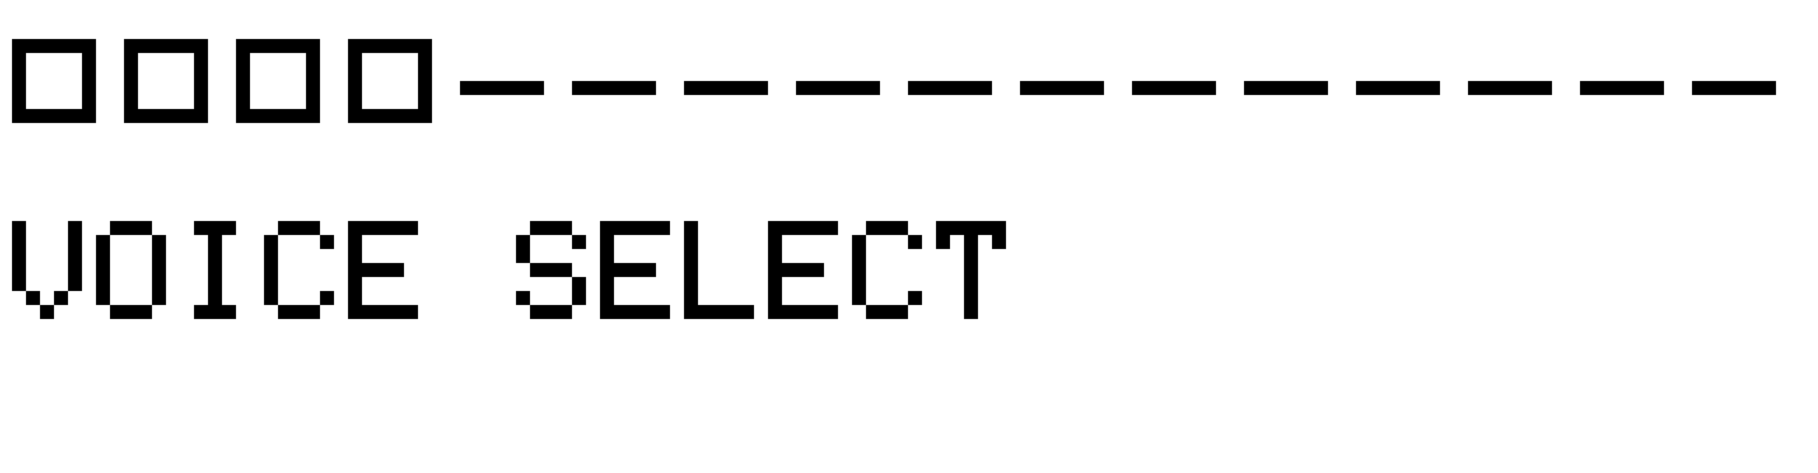
\includegraphics[scale=.40]{voice_select_page.png}}\\\\
\textit{To open the voice select page. Enter \textbf{GlobalSettings-->MD-->POLY CONFIG}}
